\section{RISMC Approach to Multi-Unit Modeling}
\label{sec:RISMC_MU_modeling}

The actual multi-unit model has been modeled using both RELAP5-3D and RAVEN.
The RELAP5-3D models the temporal response of all PWRs and SFPs while the plant 
connections and dependencies have been coded as an external model in RAVEN.
The connections between the RELAP5-3D models and the RAVEN plant model are 
shown in Fig.~\ref{fig:ensembleModel}.
Section~\ref{sec:systemModels} describes in detail the RELAP5-3D models for 
the SFPs and the PWRs while Section~\ref{sec:plantModel} describes the RAVEN plant model.
 
\begin{figure}
    \centering
    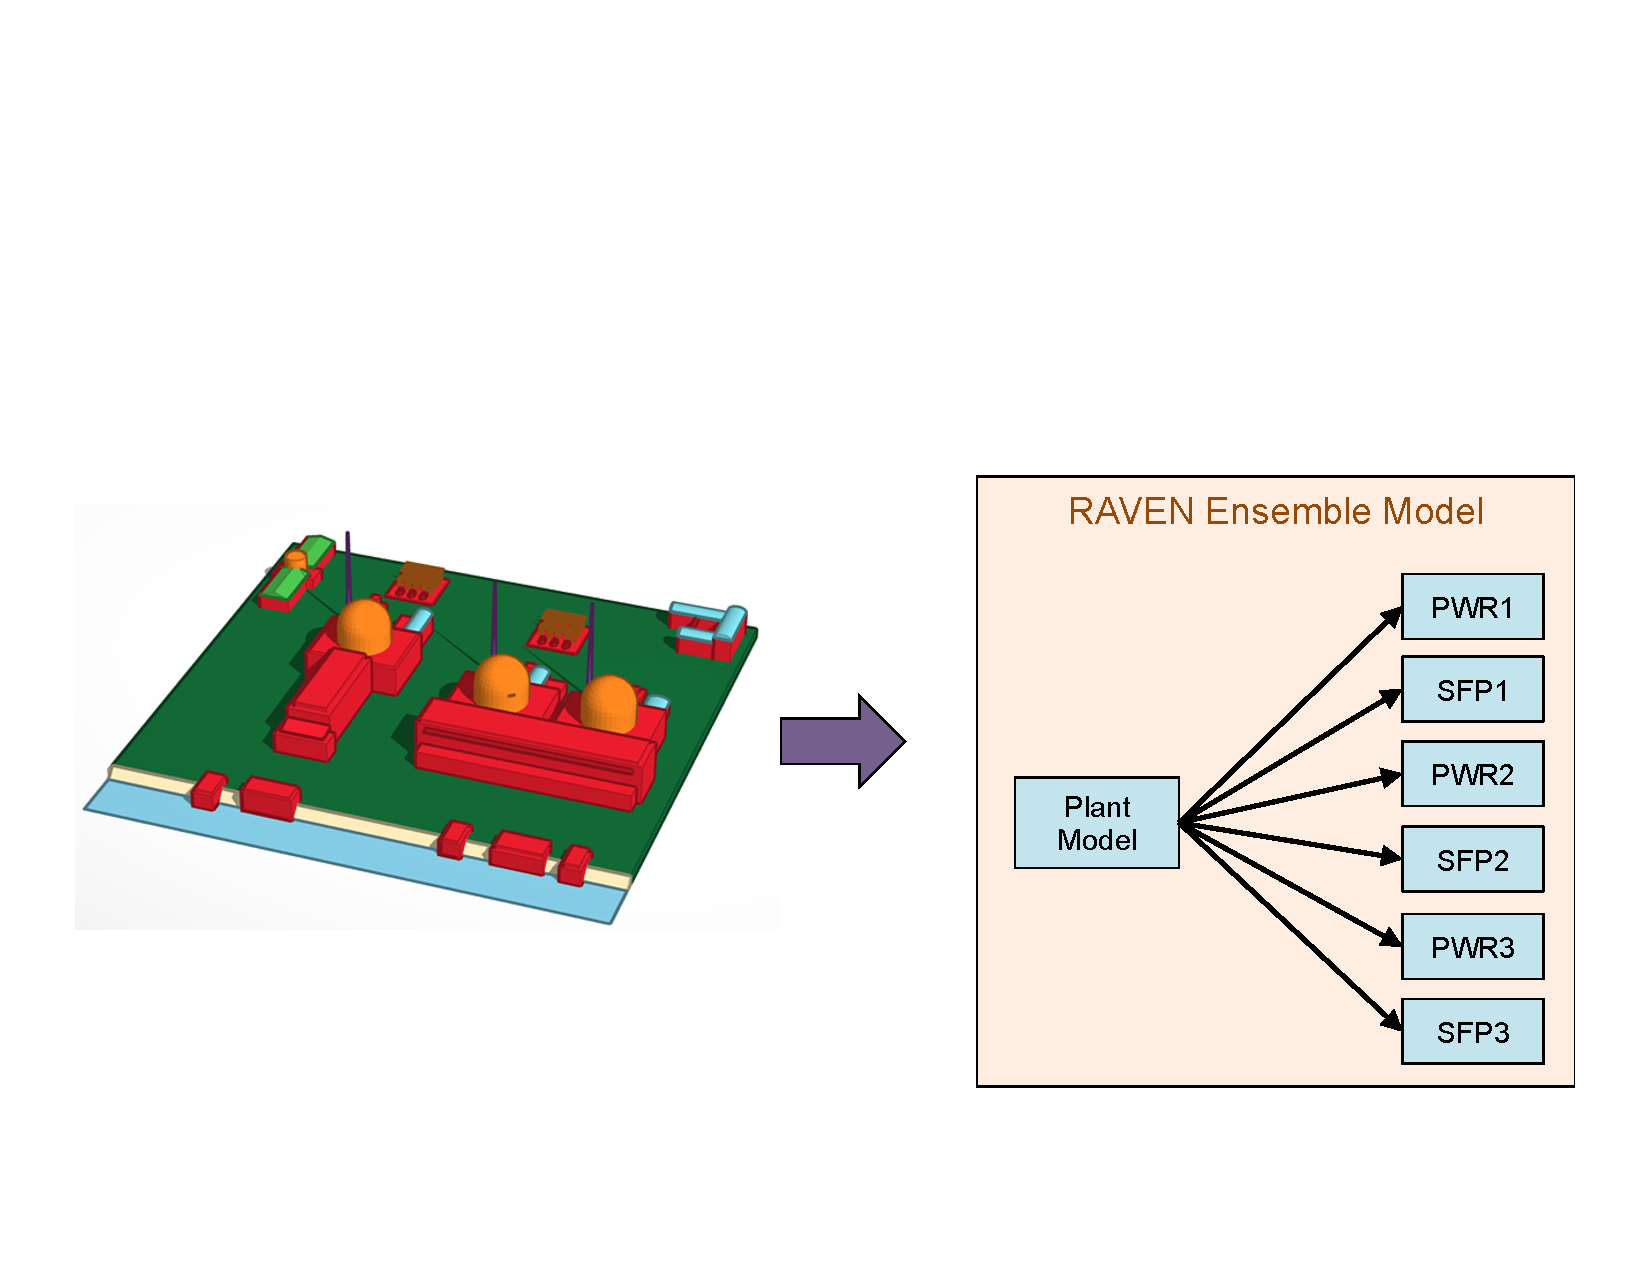
\includegraphics[scale=0.5]{ensembleModel.pdf}
    \caption{RAVEN ensemble model for the considered test case}
    \label{fig:ensembleModel}
\end{figure}

\subsection{System Models}
\label{sec:systemModels}
[CARLO]
\subsubsection{PWR1 and PWR3}

\subsubsection{PWR2}

\subsubsection{SFPs}

\subsection{Plant Model}
\label{sec:plantModel}
The plant model has been coded as a Python script and interfaced with RAVEN as an 
external model. Its main purpose is to determine timing and sequencing of events 
for all six system models (i.e., PWRs and SFPs) given the sampled values of the 
stochastic parameters.

\subsection{Human models}
To consider the performance of field workers, a simple human reliability analysis was 
performed and incorporated into the event simulation. Although many human actions are 
required, the analysis considers two human events: time to start recovery procedures 
after initiating event and EDGS involuntary alignment

Regarding the first, we employed a detailed subtask modeling using the HUNTER (Human Unimodel 
for Nuclear Technology to Enhance Reliability)~\cite{boringHUNTER} framework. The details about 
the model can be found in~\cite{hunterReport2016}; for the scope of this report, this event 
is modeled as a stochastic variable with a pdf derived from~\cite{hunterReport2016}. 

Regarding the second human related event, in order to screen the impact of the possible error, 
the human error probability 
(HEP) was obtained from the Technique for Human Error Rate Prediction (THERP) 
method~\cite{NUREGCR1278}. 
EDGS involuntary alignment corresponds well to THERP Table 20-13, Item 5: ``Making an error 
of selection in changing or restoring locally operated valve when the valve to be manipulated 
is unclearly or ambiguously labeled, part of a group of two or more valves that are similar in 
all of the following, size and shape, state, and presence of tags.'' This THERP item captures 
the nature of the task, particularly regarding complexity and ambiguity about pipe arrangements 
and corresponding valve operation. 

THERP produces an HEP equal to $1.0 10^{-2}$, with an uncertainty 
error factor of 3. THERP includes provision for considering additional degradation of performance 
due to lack of experience and situational stress. These factors were not deemed likely contributors 
to the event outcome. Event recovery was not modeled.

Thus in the analysis, we have modeled involuntary alignment of EDGS with a Bernoulli 
distribution with value of $p=1.0 10^{-2}$.

\subsection{Plant Stochastic Modeling}
\label{sec:plantStochasticModeling}
For the scope of this analysis, we have identified 23 stochastic parameters. We have 
partition this list of parameters based on their area of interest.

Regarding the SFPs, we have have identified seismic induced rupture, i.e. a SFP Loss Of
Coolant Accident (LOCA), as 
element to include into the analysis. It has been modeled by choosing two stochastic 
parameters: time of  occurrence and size of the SFP LOCA. In this work we have identified 
with locaTimeSFP1, locaTimeSFP2 and locaTimeSFP3 as the time of occurrence of the SFP 
LOCAs while locaSizeSFP1, locaSizeSFP2 and locaSizeSFP3 represents the actual size of 
the SFP LOCAs.

Regarding the PWRs, we focused on two elements: lifetime of the batteries and the LOCA 
associated to the seal of the Reactor Coolant Pumps (RCPs). Battery systems provides 
DC power to I\&C systems 
of the PWRs such as the control of the Pilot Operated Relief Valves (PORVs).
DC systems are considered for only 
Unit 1 and Unit 3; since Unit 2 is in mid-loop operation mode, its DC systems are not 
considered.

For the EDGS, we have identified the following parameters: the probability to 
involuntary align the EDGS from Unit 2 to Unit 1, the time of occurrence of EDGS
involuntary alignment and time required to perform EDGS voluntary alignment.  

Each cross-tie, CST (between Unit 2 and Unit 3), AFW (between Unit 1 and Unit 3) 
and AC (between Unit 1 and Unit 1), has been considered in the analysis and, in 
particular, they have been modeled by assigning to each of them the time required 
to perform such cross-tie.

Regarding the recovery of each unit through the EPEs, we have modeled them by 
representing them with a single stochastic parameter which represents the
time to connect the EPE to its own unit.

Lastly, the recovery plan followed by the plant crew has been modeled using a single
parameter: recovery strategy (see Section~\ref{sec:accidentProgression}).

In addition to recovery strategy, we have given an additional degree of freedom on 
the actual procedure associated to the EPE for Unit 3. 
As indicated in Section~\ref{sec:EPEactions}, depending on the  recovery strategy, 
then the EPE connection on Unit 3 can be performed in different modes. 

A summary of the chosen stochastic parameters are listed in Tables~\ref{tab:stochasticParameters1} 
and~\ref{tab:stochasticParameters2}
along a description and with their probabilistic distribution.

\begin{table}
  \centering
  \begin{center}
      \begin{tabular}{ | l | p{5cm} | c | p{5cm} |}
        \hline
         Parameter          & Description                      & Unit   & Distribution                                         \\ \hline \hline
         AUXFWxtieTime      & Time to perform AFW cross-tie    & hour   & Uniform (lower bound=.5, upper bound=1.5)            \\ \hline
         CSTxtieTime        & Time to perform CST cross-tie    & hour   & Uniform (lower bound=.5, upper bound=1.5)            \\ \hline
         recoveryStrategy   & Recovery strategy to be followed & -      & Categorical(1,2,3) (p(1)=.3, p(2)=.3, p(3)=.4)       \\ \hline
         recovProcedTime    & Time to start plant recovery procedure    & hour        & Truncated normal (mean=1., sigma=.2, lower bound=.5, upper bound=1.5)       \\ \hline
         EPETime1           & Time to connect EPE to Unit 1    & hour   & Truncated normal (mean=2., sigma=.3, lower bound=1., upper bound=3.)   \\ \hline
         EPETime2           & Time to connect EPE to Unit 2    & hour   & Truncated normal (mean=2., sigma=.3, lower bound=1., upper bound=3.)   \\ \hline
         EPETime3           & Time to connect EPE to Unit 3    & hour   & Truncated normal (mean=2., sigma=.3, lower bound=1., upper bound=3.)   \\ \hline
         EDGSinvolAlign     & Probability of occurrence for EDGS involuntary alignment & -      & Bernoulli (p=??)                               \\ \hline
         EDGSinvolAlignTime & Time of occurrence for EDGS involuntary alignment        & -      & Uniform (lower bound=.0, upper bound=1.)       \\ \hline
         EDGSswitchTime     & Time required to change EDGS alignment       & hour  & Uniform (lower bound=.25, upper bound=.75)                  \\ 
        \hline
      \end{tabular}
  \end{center}
  \caption{Summary of the stochastic parameters chosen for the multi-unit analysis and their associated distribution}
  \label{tab:stochasticParameters1}
\end{table}

\begin{table}
  \centering
  \begin{center}
      \begin{tabular}{ | l | p{5cm} | c | p{5cm} |}
        \hline
         Parameter          & Description                      & Unit      & Distribution                                         \\ \hline \hline
         ACxTieUnit12       & Time to perform AC cross-tie     & hour      & Uniform (lower bound=.5, upper bound=1.)             \\ \hline
         batteryTime1       & Battery life for Unit 1          & hour      & Triangular (lower bound=6., upper bound=8., peak=7.) \\ \hline
         batteryTime3       & Battery life for Unit 3          & hour      & Triangular (lower bound=6., upper bound=8., peak=7.) \\ \hline
         locaTimePWR1       & Time of occurrence for PWR1 seal LOCA & hour & Uniform (lower bound=.1667, upper bound=.25)         \\ \hline
         locaTimePWR3       & Time of occurrence for PWR3 seal LOCA & hour & Uniform (lower bound=.1667, upper bound=.25)         \\ \hline
         locaSizeSFP1       & LOCA size for SFP1               & gpm       & Categorical(0.0004,0.0035,0.056) (p(0.0004)=.85, p(0.0035)=.1, p(0.056)=.05)   \\ \hline
         locaSizeSFP2       & LOCA size for SFP1               & gpm       & Categorical(0.0004,0.0035,0.056) (p(0.0004)=.85, p(0.0035)=.1, p(0.056)=.05)   \\ \hline
         locaSizeSFP3       & LOCA size for SFP1               & gpm       & Categorical(0.0004,0.0035,0.056) (p(0.0004)=.85, p(0.0035)=.1, p(0.056)=.05)   \\ \hline    
         locaTimeSFP1       & Time of occurrence for SFP1 LOCA & hour      & Categorical(0.,.1667,.333,.5,24.) (p(0.)=.025, p(.1667)=.025, p(.333)=.025, p(.5)=.025, p(24.)=.9)  \\ \hline
         locaTimeSFP2       & Time of occurrence for SFP2 LOCA & hour      & Categorical(0.,.1667,.333,.5,24.) (p(0.)=.025, p(.1667)=.025, p(.333)=.025, p(.5)=.025, p(24.)=.9)  \\ \hline
         locaTimeSFP3       & Time of occurrence for SFP3 LOCA & hour      & Categorical(0.,.1667,.333,.5,24.) (p(0.)=.025, p(.1667)=.025, p(.333)=.025, p(.5)=.025, p(24.)=.9)  \\ \hline
         flex3Strategy13    & Type of EPE connection for Unit 3 during recovery strategy 1 and 3  & -      & Categorical(1,2) (p(1)=.3, p(2)=.7)             \\ \hline
         flex3Strategy2     & Type of EPE connection for Unit 3 during recovery strategy 2        & -      & Categorical(1,2) (p(1)=.4, p(2)=.6)             \\ 
        \hline
      \end{tabular}
  \end{center}
  \caption{Summary of the stochastic parameters chosen for the multi-unit analysis and their associated distribution (cont.)}
  \label{tab:stochasticParameters2}
\end{table}


